\documentclass[11pt]{article}
\usepackage[sc]{mathpazo}
\usepackage{amsmath,pifont}
\usepackage{fullpage}
\usepackage[authoryear,sectionbib,sort]{natbib}
\linespread{1.7}
\usepackage[utf8]{inputenc}
\usepackage{lineno}

\usepackage{graphicx} 
\usepackage{tabularx,setspace}

\title{Density-dependent selection in evolutionary genetics: a lottery model of Grime's triangle}
%\author{Jason Bertram $^{1,\ast}$ \\ 
%Joanna Masel $^{1}$}

\date{}

\begin{document}

\maketitle

%\noindent{}1. Department of Ecology and Evolutionary Biology, University of Arizona, Tucson, AZ 85721.

%\noindent{}$\ast$ Corresponding author; e-mail: jbertram@email.arizona.edu.


\bigskip

\textit{Manuscript elements}: 

\bigskip

\textit{Keywords}: r/K selection, absolute fitness, eco-evo, interference competition, competition-colonization trade-off.

\bigskip

\textit{Manuscript type}: Article. 
% Or e-article, note, e-note, natural history miscellany,
% e-natural history miscellany, comment, reply, symposium, or
% countdown to 150.

\bigskip

\noindent{\footnotesize Prepared using the suggested \LaTeX{} 
template for \textit{Am.\ Nat.}}

\linenumbers{}
\modulolinenumbers[3]

\newpage{}

\section*{Abstract}

Fitness is typically represented in heavily simplified terms in evolutionary genetics, often using constant selection coefficients. This excludes fundamental ecological factors such as dynamic population size or density-dependence from the most genetically-realistic treatments of evolution, a problem that inspired MacArthur's influential but problematic $r$/$K$ theory. Following in the spirit of $r$/$K$-selection as a general-purpose theory of density-dependent selection, but grounding ourselves empirically in ``primary strategy'' trait classification schemes like Grime's triangle, we develop a new model of density-dependent selection which revolves around territorial contests. To do so, we generalize the classic lottery model of territorial acquisition, which has primarily been used for studying species co-existence questions, to accommodate arbitrary densities. We use this density-dependent lottery model to predict the direction of trait evolution under different environmental conditions and thereby provide a mathematical underpinning for Grime's verbal scheme. We revisit previous concepts of density-dependent selection, including $r$ and $K$ selection, and argue that our model distinguishes between different aspects of fitness in a more natural and intuitive manner.

\newpage{}

``...the concept of fitness is probably too complex to allow of a useful mathematical development. Since it enters fundamentally into many population genetics considerations, it is remarkable how little attention has been paid to it.'' --- Warren J. Ewens, Mathematical Population Genetics I, 2004 

Evolutionary models differ greatly in their treatment of fitness. In models of genetic evolution, genotypes are typically assigned constant (or frequency-dependent) selection coefficients describing the change in their relative frequencies over time due to differences in viability. This considerably simplifies the mathematics of selection, facilitating greater genetic realism, and can be justified over sufficiently short time intervals \citep[p. 276]{ewens_2004}. However, the resulting picture of evolution does not include even basic elements of the ecological underpinnings of selection, including dynamic population size and density-dependence.

By contrast, models of phenotypic trait evolution represent the change in phenotypic abundances over time using absolute fitness functions which describe how those traits affect survival and reproduction in particular ecological scenarios. This approach is powerful enough to model eco-evolutionary feedbacks between co-evolving traits, but is generally problem-specific and restricted to only a few traits at a time.

Far less work has been done to generalize beyond particular traits or ecological scenarios to models of fitness that still capture key distinctions between different forms of selection. Perhaps this is not surprising given that fitness is such a complex quantity, dependent on all of a phenotype's functional traits \citep{violle_2007} as well as its biotic and abiotic environment. In most cases, a detailed, trait-based, predictive model of fitness would be enormously complicated and have narrow applicability. It is therefore easy to doubt the feasibility of a simplified, general mathematical treatment of fitness \citep[p. 276]{ewens_2004}. For example, MacArthur's famous $r$/$K$ scheme \citep{macarthur_1962,macarthur_1967} is now almost exclusively known as a framework for understanding life-history traits, and judged on its failure in that role \citep{pianka_1970,stearns_1977,boyce_1984,reznick_2002}. The r/K scheme's original purpose was as an extension of the existing population-genetic treatment of selection to account for population density \citep{macarthur_1962}, but few attempts have been made to develop it further as a mathematical analysis of the major different forms of selection. 

Nevertheless, there are strong indications there exist broader principles governing the operation of selection. In many groups of organisms, including corals \citep{darling_2012}, insects \citep{southwood_1977}, fishes \citep{winemiller_1992}, zooplankton \citep{allan_76} and plants \citep{grime_1988,westoby_1998}, different species can be divided into a small number of distinct trait clusters corresponding to fundamentally distinct ``primary strategies'' \citep{winemiller_2015}. The most famous example is Grime's plant trait classification scheme \citep{grime_1974,grime_1977,grime_1988}. Grime considered two broad determinants of population density: stress (persistent hardship e.g. due to resource scarcity, unfavorable temperatures or toxins) and disturbance (intermittent destruction of vegetation e.g. due to trampling, herbivory, pathogens, extreme weather or fire).  The extremes of these two factors define three primary strategies denoted by C/S/R respectively (Fig. \ref{fig:grimeschematic}): competitors ``C'' excel in low stress, low disturbance environments; stress tolerators ``S'' excel in high stress, low disturbance environments; and ruderals ``R''  excel in low stress, high disturbance environments. Survival is not possible in high-stress, high-disturbance environments. Grime showed that measures of C, S and R across a wide range of plant species are anti-correlated, so that strong C-strategists are weak S and R strategists, and so on. Thus, plant species can be classified on a triangular C/S/R ternary plot \citep{grime_1974}. Trait classification schemes for other organisms are broadly analogous to Grime's scheme \citep{winemiller_2015}. 

\begin{figure}
\centering
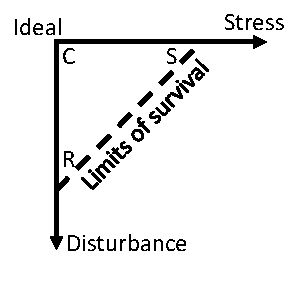
\includegraphics[scale=1]{grimeschematic.pdf}
\caption{\label{fig:grimeschematic} Schematic of Grime's triangle. The two axes show increasing levels of environmental stress and disturbance, respectively. Survival is not possible if the combination of stress and disturbance is too large (dashed line). This creates a triangle, each corner of which corresponds to a ``primary strategy''.} 
\end{figure}

Trait classification schemes show empirically that, beneath the complicated details of trait variation, even among closely-related species, fitness is predominantly determined by a few key factors such as intrinsic reproductive rate or stress-tolerance. However, while trait classification schemes are firmly grounded in trait data, they are verbal and descriptive rather than mathematical, a recognized hindrance to their broader applicability (e.g. \citealt{tilman_2007}). 

The aim of this paper is explore the interplay between some major dimensions of fitness in a simplified, territorial model of growth, dispersal and competition. Building on the earlier r/K and C/S/R schemes, a central question is how fitness depends on the interaction between population density, intrinsic birth/death rates and competitive ability. 

We broadly follow the spirit of MacArthur's $r$/$K$ selection scheme in that our model is intended to account for fundamentally different forms of selection without getting  entangled in the intricacies of particular ecological scenarios. However, rather than building directly on MacArthur's formalism and its later extensions using Lotka-Volterra equations to incorporate competition (``$\alpha$-selection'') \citep{gill_1974,case_1974,joshi_2001}, our model is devised more with Grime's C/S/R scheme in mind, and represents a quantitative formalization of how C/S/R manifests at the level of within-population genotypic evolution (as opposed to phenotypic divergence between species). This choice is motivated in part by the substantial empirical support for C/S/R-like schemes, and in part by the failings of the $r$/$K$ low/high density dichotomy --- many growth ability traits will confer advantages at both low and high densities (more details in the Discussion). 

As we will see, a generalized version of the classic lottery model of \cite{chesson_1981} is a convenient starting point for ecologically-grounded models of selection in evolutionary genetics. In the classic lottery model, mature individuals (``adults'') each require their own territory, whereas newborn individuals (``propagules'') disperse to, and subsequently compete for, territories made available by the death of adults. Territorial contest among propagules leaves a single victorious adult per territory, the victor chosen at random from the propagules present (akin to a lottery; \citealt{sale_77}), with probabilities weighted by a coefficient for each type representing competitive ability. This representation of competition is much simpler than having coefficients for the pairwise effects of types on each other (e.g. the $\alpha$ coefficients in the generalized Lotka-Volterra equations), or than modeling resource consumption explicitly \citep{tilman_1982}. The classic lottery model is also closely connected to one of the central models of population genetics, the Wright-Fisher model of genetic drift. 

However, the classic lottery model breaks down at low densities (that is, if there are only a few propagules dispersing to each territory; see ``Model''). This was not a limitation in the lottery model's original application to reef fishes, where a huge number of larvae from each species compete to secure territories each generation \citep{chesson_1981}, but is a critical limitation for studying density-dependent selection. We analytically extend the classic lottery model to correctly account for low density behavior. 

In the section ``Model'', we introduce the basic assumptions of our generalized lottery model. Analytical expressions for the change in genotype abundances over time are introduced in section ``Mean field approximation'', with mathematical details relegated to the Appendices. In the following two sections, we then discuss the behavior of rare mutants (invasion and coexistence) and our formalization of Grime's triangle. 
 
\section*{Model}\label{sec:model}

We assume that the reproductively mature individuals in a population (``adults'') each require their own territory to survive and reproduce (Fig.~\ref{fig:lottery}). All territories are identical, and the total number of territories is $T$. Time $t$ advances in discrete iterations, each representing the average time from birth to reproductive maturity. In iteration $t$, the number of adults of the $i$'th genotype is $n_i(t)$, the total number of adults is $N(t)=\sum_i n_i(t)$, and the number of unoccupied territories is $U(t)=T-N(t)$. 

\begin{figure}
\centering
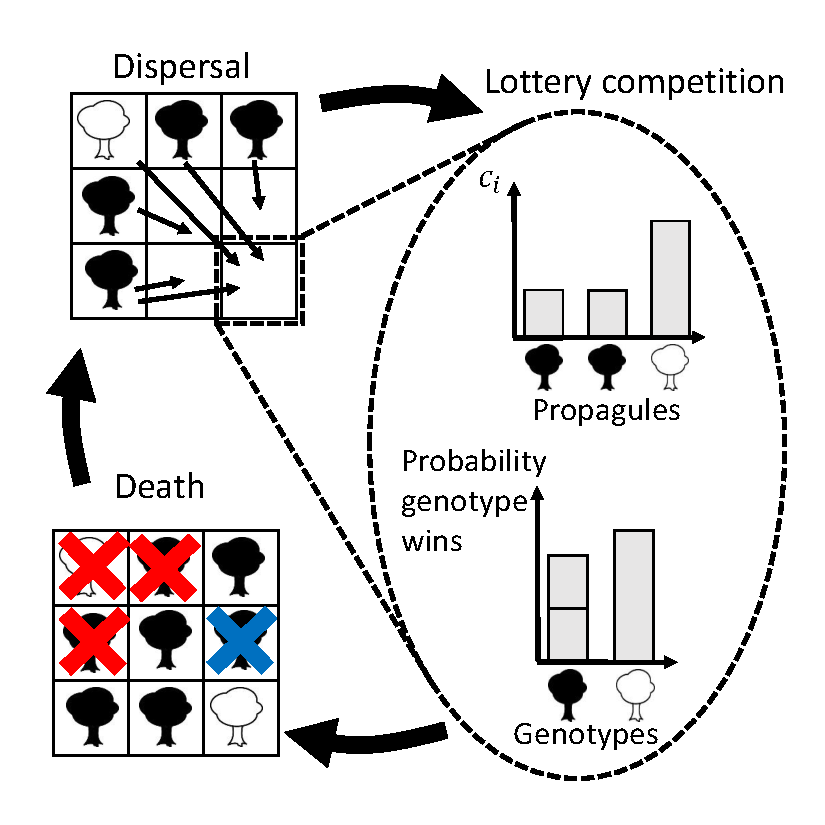
\includegraphics[scale=0.8]{lottery.pdf}
\caption{\label{fig:lottery} Each iteration of our lottery model has three main elements. First, propagules are produced by adults which are dispersed at random over the unoccupied territories (only propagules landing on unoccupied territories are shown). Lottery competition then occurs in each unoccupied territory (competition in only one territory is illustrated): each genotype has a probability proportional to $b_i n_i c_i$ of securing the territory. Then occupied territories are freed up by adult mortality. In Eq. \eqref{eq:delttot} and most of the paper, only adults can die (red crosses), but we will also consider the case where juveniles die (blue cross; section ``Primary strategies and Grime's triangle'').}
\end{figure}

Each iteration, adults produce new offspring (``propagules''), $m_i$ of which disperse to unoccupied territories. We assume that adults cannot be ousted from occupied territories, and so only propagules landing on unoccupied territories are included in $m_i$. Propagules disperse at random uniformly, and independently of each other; all propagules have the same probability of landing on any of the $U$ unoccupied territories. Thus, there is no interaction between propagules (e.g. avoidance of territories crowded with propagules). Loss of propagules during dispersal is subsumed into $m_i$. In general, $m_i$ will increase with $n_i$, and will also depend on population density $N$. For example, if $b_i$ is the number of successfully dispersing propagules produced per genotype $i$ adult, then the loss of propagules due to dispersal to occupied territories implies $m_i=b_i(1-N/T)n_i$, akin to Levins' competition-colonization model \citep{levins_71,tilman_94}. Here we assume $m_i=b_i n_i$, where $b_i$ is a constant, meaning that all propagules land on unoccupied territories (a form of directed dispersal). This choice simplifies the mathematics without seriously restricting the generality of our analysis, since the results presented here are not sensitive to the specific functional form of $m_i$. Note that due to our assumption of uniform dispersal, the parameter $b_i$ can be thought of as a measure of ``colonization ability'', which combines fecundity and dispersal ability \citep{levins_71,tilman_94,bolker_99}. 

The number of individuals of the $i$'th genotype landing in any particular territory is denoted $x_i$. Random dispersal implies that in the limit $T\rightarrow \infty$, with $n_i/T$ held fixed, $x_i$ is Poisson distributed with mean territorial propagule density $l_i=m_i/U$ (this dispersal Poisson distribution is denoted $p_i(x_i)=l_i^{x_i} e^{-l_i}/x_i!$). Although $T$ is finite in our model, we assume that $T$ and the $n_i$ are large enough that $x_i$ is Poisson-distributed to a good approximation (details in Appendix A). Note that the large $n_i$, large $T$ approximation places no restrictions on our densities $n_i/T$, but it does preclude consideration of demographic stochasticity when $n_i$ itself is very small.

When multiple propagules land on the same territory, they compete to secure the territory as they develop. This territorial contest is modeled as a weighted lottery: the probability that genotype $i$ wins a territory by the next iteration, assuming that at least one of its propagules is present, is $c_i x_i/\sum_j c_j x_j$, where $c_i$ is a constant representing relative competitive ability (Fig. \ref{fig:lottery}). 

In the classic lottery model \citep{chesson_1981}, unoccupied territories are assumed to be saturated with propagules from every genotype i.e. $l_i\gg 1$ where $l_i=m_i/U$ is the mean propagule density. From the law of large numbers, the composition of propagules in each territory will then not deviate appreciably from the mean composition $l_1,l_2,\ldots,l_G$ ($G$ is the number of genotypes present), and so the probability that genotype $i$ wins any particular unoccupied territory is approximately $c_i l_i/\sum_j c_j l_j$. Let $\Delta_+ n_i$ denote the number of territories won by genotype $i$. Then $\Delta_+ n_1,\Delta_+ n_2,\ldots,\Delta_+ n_G$ follow a multinomial distribution with $U$ trials and success probabilities $\frac{c_1 l_1}{\sum_j c_j l_j},\frac{c_2 l_2}{\sum_j c_j l_j},\ldots,\frac{c_G l_G}{\sum_j c_j l_j}$, respectively. Genotype $i$ is expected to win $c_i l_i/\sum_j c_j l_j$ of the $U$ available territories, and deviations from this expected outcome are small (since $T$ is large by assumption), giving 
\begin{equation}
\Delta_+ n_i(t)=\frac{c_i l_i}{\sum_j c_j l_j}U(t)=b_i n_i\frac{1}{L}\frac{c_i}{\overline{c}}, \label{eq:lottery}
\end{equation}
where $\overline{c}=\sum_j c_j m_j/M$ is the mean propagule competitive ability for a randomly selected propagule, $L=M/U$ is the total propagule density and $M=\sum_j m_j$ is the total number of propagules. 

There is a close connection between the classic lottery model and the Wright-Fisher model of genetic drift \citep{svardal_2015}. In the Wright-Fisher model, genotype abundances are sampled each generation from a multinomial distribution with success probabilities $w_i n_i/\sum_j w_j n_j$, where $w$ is relative fitness and the $n_i$ are  genotype abundances in the preceding generation. Population size $N$ remains constant. This is mathematically equivalent to the classic lottery model with non-overlapping generations ($d_i=1$ for all $i$) and $w_i=b_i c_i$. 

The classic lottery model allows us to replace the abstract Wright-Fisher relative fitnesses $w_i$ with more ecologically-grounded fecundity, competitive ability and mortality parameters $b_i$, $c_i$ and $d_i$, respectively. Since birth and death rates affect absolute abundances, this allows us to evaluate selection at different densities (after appropriate extensions are made), in an otherwise very similar model to the canonical Wright-Fisher model. Note that the classic lottery model, and the present work, both ignore the stochastic drift in type frequencies (large $T$ approximation) which is the focus of the Wright-Fisher model. 

In our extension of the classic lottery model, we do not restrict ourselves to high propagule densities. Eq. \eqref{eq:lottery} is nonsensical at low densities ($l_i\ll 1$): genotype $i$ can win at most $m_i$ territories, yet Eq. \eqref{eq:lottery} demands $c_i l_i/\sum_j c_j l_j$ of the $U$ unoccupied territories, for any value of $U$. Intuitively, the cause of this discrepancy is that individuals are discrete. Genotypes with few propagules depend on the outcome of contests in territories where they have at least one propagule present, not some small fraction of a propagule as would be implied by low propagule density $l$ in the classic lottery model. In other words, deviations from the mean propagule composition $l_1,l_2,\ldots,l_G$ are important at low density. 

Dispersal is Poisson, and so we expect that a fraction $p_1(x_1)\ldots p_G(x_G)$ of the $U$ unoccupied territories will have the propagule composition $x_1,\ldots,x_G$. Genotype $i$ is expected to win $c_i x_i/\sum_j c_j x_j$ of these. Ignoring fluctuations about these two expectations (large $T$ approximation), genotype $i$'s territorial acquisition is given by
\begin{equation}
\Delta_+ n_i(t)=U(t)\sum_{x_1,\ldots,x_G} \frac{c_i x_i}{\sum_j c_j x_j} p_1(x_1)\ldots p_G(x_G), \label{eq:growthsumuncoupled}
\end{equation}
in our extended lottery model, where the sum only includes territories with at least one propagule present. 

For the majority of this manuscript we assume that mortality only occurs in adults (setting aside the juvenile deaths implicit in territorial contest), and at a constant, genotype-specific per-capita rate $d_i$, so that the overall change in genotype abundances is
\begin{equation}
\Delta n_i(t)=\Delta_+ n_i(t)-d_i n_i(t). \label{eq:delttot}
\end{equation}
This is reasonable approximation in the absence of disturbances; when we come to consider the effects of disturbances (Section ``Primary strategies and Grime's triangle''), we will incorporate disturbance-induced mortality in competing juveniles (Fig.~\ref{fig:lottery}). 

Note that the competitive ability coefficients $c_i$ represent a strictly relative aspect of fitness in the sense that they can only influence population size $N$ indirectly by changing genotype frequencies. This can be seen by summing Eq. \eqref{eq:delttot} over genotypes to get the  change in population size $N$, 
\begin{equation}
\Delta N=U(1-e^{-L})-\sum_i d_i n_i,\label{eq:deltN}
\end{equation}
which is independent of $c_i$ (here $L=\sum_j l_j$ is the overall propagule density). Unlike the classic lottery model, not all $U$ unoccupied territories are claimed each iteration; a fraction $e^{-L}$ remain unoccupied.

\section*{Results}

\subsection*{Mean Field Approximation}

Eq. \eqref{eq:growthsumuncoupled} involves an expectation over the time-dependent dispersal distributions $p_i$, and is thus too complicated to give intuition about the dynamics of density-dependent lottery competition. We now evaluate this expectation using a ``mean field'' approximation. 

Our approximation is similar to the high-$l_i$ approximation behind the classic lottery model in that we replace the $x_i$ with appropriate mean values. However, we cannot simply replace $x_i$ with $l_i$ as in the classic lottery model. For a genotype with a low propagule density $l_i\ll 1$, we have $x_i=1$ in the few territories where its propagules land, and so its growth comes entirely from territories which deviate appreciably from $l_i$. In our more general approximation, territories with a single propagule from the focal genotype are handled separately. In place of the requirement of $l_i\gg 1$ for all $i$, our approximation only requires that there are no large discrepancies in competitive ability (specifically, that we do not have $c_i/c_j\gg 1$ for any two genotypes; further discussion in section ``Discussion''). We obtain (details in Appendix B)
\begin{equation}
\Delta_+ n_i(t)\approx b_i n_i\left[e^{-L}+(R_i+A_i)\frac{c_i}{\overline{c}}\right], \label{eq:master}
\end{equation}
where
\begin{equation}
R_i=\frac{\overline{c}e^{-l_i}(1-e^{-(L-l_i)})}{c_i +\frac{L-1+e^{-L}}{1-(1+L)e^{-L}}\frac{\overline{c}L- c_il_i}{L-l_i}},\label{eq:Dr}
\end{equation}
and
\begin{equation}
A_i=\frac{\overline{c}(1-e^{-l_i})}{\frac{1-e^{-l_i}}{1-(1+l_i)e^{-l_i}}c_il_i+\frac{1}{L-l_i}\left(L\frac{1-e^{-L}}{1-(1+L)e^{-L}}-l_i\frac{1-e^{-l_i}}{1-(1+l_i)e^{-l_i}}\right)\sum_{j\neq i}c_jl_j}.\label{eq:Da}
\end{equation}

Comparing Eq. \eqref{eq:master} to Eq. \eqref{eq:lottery}, the classic lottery per-propagule success rate $c_i/\overline{c}L$ has been replaced by three separate terms. The first, $e^{-L}$, accounts for propagules which land alone on unoccupied territories; these territories are won without contest. The second, $R_i c_i/\overline{c}$ represents competitive victories when the $i$ genotype is a rare invader in a high density population: from Eq. \eqref{eq:Dr}, $R_i\rightarrow 0$ when the $i$ genotype is abundant ($l_i\gg 1$), or other genotypes are collectively rare ($L-l_i\ll 1$). The third term, $A_ic_i/\overline{c}$, represents competitive victories when the $i$ genotype is abundant: $A_i\rightarrow 0$ if $l_i\ll 1$. The relative importance of these three terms varies with both the overall propagule density $L$ and the relative propagule frequencies $m_i/M$. If $l_i\gg 1$ for all genotypes, we recover the classic lottery model (only the $A_ic_i/\overline{c}$ term remains, and $A_i\rightarrow 1/L$). Thus, Eq. \eqref{eq:master} generalizes the classic lottery model to account for arbitrary propagule densities for each genotype. 

Fig.~\ref{fig:simcomp} shows that Eq. \eqref{eq:master} (and its components) closely approximate direct simulations of random dispersal and lottery competition over a wide range of propagule densities (obtained by varying $U$). Two genotypes are present, one of which has a $c$-advantage and is at low frequency. The growth of the low-frequency genotype relies crucially on the low-density competition term $R_i c_i/\overline{c}$, and also to a lesser extent on the high density competition term $A_i c_i/\overline{c}$ if $l_1$ is large enough (Fig.~\ref{fig:simcomp}b). On the other hand, $R_i c_i/\overline{c}$ is negligible for the high-frequency genotype, which depends instead on high density territorial victories (Fig.~\ref{fig:simcomp}d). Fig. 3 also shows the breakdown of the classic lottery model at low densities (low $l_1$ and $l_2$).

\begin{figure}
\centering
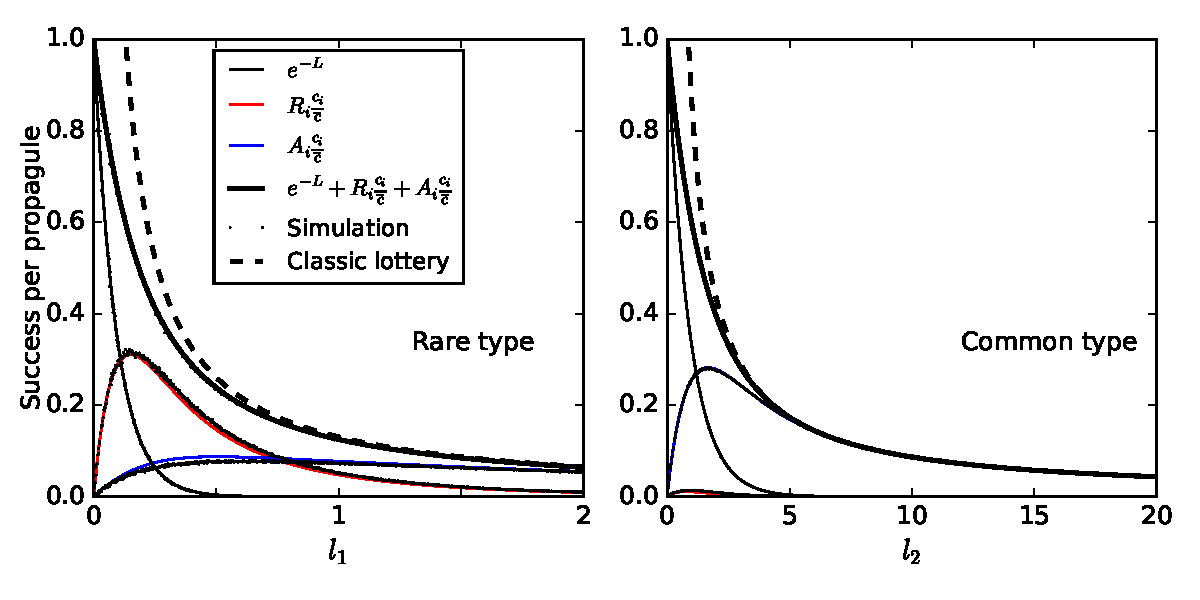
\includegraphics[scale=0.7]{simulationcomparison.pdf}
\caption{\label{fig:simcomp} The change in genotype abundances in a density dependent lottery model is closely approximated by Eq. \eqref{eq:master}. $\Delta_+ n_i/m_i$ from Eq. \eqref{eq:master} (and its separate components) are shown, along with direct simulations of random dispersal and lottery competition over one iteration over a range of propagule densities (varied by changing $U$ with the $m_i$ fixed). Two genotypes are present. (a) and (b) show the low-frequency genotype with $c$-advantage ($m_1/M=0.1$, $c_1=1.5$), (c) and (d) show the high-frequency predominant genotype ($m_2/M=0.9$, $c_2=1$). Simulation points are almost invisible in (c) and (d) due to near exact agreement with Eq. \eqref{eq:master}. Dashed lines in (a) and (c) show the corresponding classic lottery model predictions.} 
\end{figure}


\subsection*{Invasion of rare genotypes and coexistence}\label{sec:invas}

In our model (section ``Model''), each genotype is defined by three traits: $b$, $c$ and $d$. To determine how these will evolve in a population where they are being modified by mutations, we need to know whether mutant lineages will grow (or decline) starting from low densities. In this section we discuss the behavior of rare genotypes predicted by Eq. \eqref{eq:master}. 

Suppose that a population with a single genotype $i$ is in equilibrium. Then $R_i=0$, $\overline{c}=c_i$ and $\Delta n_i = 0$, and so Eq. \eqref{eq:master} gives
\begin{equation}
b_i\left(e^{-L}+A_i\right)-d_i=0,\label{eq:equil}
\end{equation}
where $A_i=(1-(1+L)e^{-L})/L$. Now suppose that a new genotype $j$, which is initially rare, appears in the population. Then $A_j\ll R_j$, $l_j\approx 0$ and $\overline{c}\approx c_i$, and so, from Eq. \eqref{eq:master}, $n_j$ will increase if 
\begin{equation}
b_j \left(e^{-L}+R_j\frac{c_j}{c_i}\right)-d_j>0,\label{eq:invad}
\end{equation}
where $R_j\approx (1-e^{-L})/\left(\frac{c_j}{c_i}+\frac{L-1-e^{-L}}{1-(1+L)e^{-L}}\right)$. 

Combining Eqs. \eqref{eq:equil} and \eqref{eq:invad}, we see that $j$ will invade if it is superior in any one of the three traits, but is otherwise identical to $i$. If the new genotype has the same competitive ability $c_j=c_i$, then $R_j\approx A_i$ and Eqs. \eqref{eq:equil} and \eqref{eq:invad} imply that invasion occurs when $b_jd_i-b_id_j>0$, and in particular when $b_j>b_i$ with $d_j=d_i$, or when $d_j<d_i$ with $b_j=b_i$. In the case that the new genotype has a different competitive ability but the same $b_i$ and $d_i$, Eqs. \eqref{eq:equil} and \eqref{eq:invad} imply that invasion occurs when $R_j c_j/c_i > A_i$; it is not hard to verify that this occurs if and only if $c_j>c_i$ using the simplified expressions for $A_i$ and $R_j$ given after Eqs. \eqref{eq:equil} and \eqref{eq:invad} respectively. Moreover, if $j$ invades in any of these cases, it will eventually exclude $i$, since it is strictly superior. 

Stable coexistence is possible between genotypes that are superior in different traits. Suppose that $j$ is better at securing territories ($c_j>c_i$), that $i$ is better at producing propagules ($b_i>b_j$), and that $d_i=d_j$. Coexistence occurs if $j$ will invade an $i$-dominated population, but $i$ will also invade a $j$-dominated population (``mutual invasion''). If $b_i$ is so large that $L\gg 1$ when $i$ is dominant, and $b_j$ is so small that $L\ll 1$ when $j$ is dominant, then, combining Eqs. \eqref{eq:equil} and \eqref{eq:invad}, we find that $i$ invades $j$ because $b_i>b_j$, while $j$ invades $i$ provided that
\begin{equation}
b_jc_jR_j-b_i c_i A_i>0. \label{eq:jinvadcoex}
\end{equation}
Thus, coexistence occurs if $c_j/c_i$ is large enough. This is a version of the classic competition-colonization trade-off \citep{tilman_94,levins_71}: the competitor ($c$-specialist) leaves many territories unoccupied (low $L$) due to its poor colonization ability (low $b$), which the colonizer ($b$-specialist) can then exploit. A similar argument applies for coexistence between high-$c$ and low-$d$ specialists; a ``competition-longevity'' trade-off \citep{tilman_94}. Mutual invasibility is not possible between $b$- and $d$-specialists. 

If the rare genotype $j$ arises due to mutation, then its initial low-density behavior is more complicated than the above invasion analysis suggests. The mutant lineage starts with one individual $n_j=1$, and remains at low abundance for many generations after its initial appearance. During this period, the mutant abundance $n_j$ will behave stochastically, and the deterministic equations \eqref{eq:growthsumuncoupled} and \eqref{eq:master} do not apply (section ``Model''). However, if $n_j$ becomes large enough, its behavior will become effectively deterministic, and governed by Eq. \eqref{eq:master}. For mutants with fitness greater than the population mean fitness, this occurs when $n_j$ is of order $1/s$ \citep{desai_2007}, where the selection coefficient $s$ is the mutant's fitness advantage (i.e. $s=\frac{\Delta n_i/n_i}{\sum_i\Delta n_i/n_i\times n_i/N}-1$). Here we do not consider the initial stochastic behavior of novel mutants, and have restricted our attention to the earliest deterministic behavior of rare genotypes. In particular, for beneficial mutations we have only considered the case where $s$ is large enough that deterministic behavior starts when $n_j \ll N$.

\subsection*{Primary strategies and Grime's triangle}

We now discuss which changes in the traits $b, c$ and $d$ will be particularly favored under different environmental conditions. Of specific interest are Grime's ``disturbed'', ``stressful'' and ``ideal'' environments. To proceed, we need to map these verbally-defined environments to quantitative parameter regimes in our model. 

The ideal environment is characterized by the near-absence of stress and disturbance. Consequently, $d_i\ll 1$, whereas $b_i$ is potentially much larger than $1$. From Eq. \eqref{eq:deltN}, the equilibrium value of $L$ only depends on the ratio of birth and death rates. For one genotype, $L/(1-e^{-L})=b_i/d_i$, and so the propagule density is high $L\approx b_i/d_i\gg 1$, and every unoccupied territory will be heavily contested. The population density is also high $N/T\approx 1$ (since $L=b_iN/(N-T)=b_i/(1-T/N)$). 

Disturbed environments are characterized by unavoidably high extrinsic mortality caused by physical destruction. Environmental variability, and disturbances in particular, can be modeled as stochastic fluctuations in $b$, $c$ and $d$ \citep{chesson_1981}. For simplicity, we do not pursue this more complicated stochastic approach. Instead, we represent disturbance by high constant mortality rates $d_i$, and extend this mortality to juveniles in the process of territorial contest (since disturbances do not only affect adults as in Eq. \eqref{eq:delttot}). We assume that disturbances are equally damaging to adults and juveniles, so that only $(1-d_i)\Delta_+ n_i$ rather than $\Delta_+ n_i$ territories are secured by genotype $i$ each iteration. [More justification?] Disturbed environments then correspond to $d_i$ being close to $1$ for all genotypes (almost all adults and juveniles are killed each iteration). From Eq. \eqref{eq:deltN}, the single genotype equilibrium is given by $L/(1-e^{-L})=d_i/[(1-d_i)b_i]$, and since $L\ll 1$ and $N/T\ll 1$ due to high mortality, we have $L\approx 2(1-d_i/[(1-d_i)b_i])$. Clearly $b_i$ must be exceptionally large to ensure population persistence. The terms proportional to $c_i/\overline{c}$ in Eq. \eqref{eq:master} are then negligible, and $\Delta_+ n_i$ depends primarily on $b_i$. 

Stressful environments are more ambiguous, and have been the subject of an extensive debate in the plant ecology literature (the ``Grime-Tilman'' debate; \citealt{aerts_1999} and references therein). Severe stress inhibits growth and reproduction, so that $b\ll 1$ \citep{grime_1974,grime_1977}. Mutations which appreciably improve $b$ will be either non-existent or extremely unlikely, so $b$ is constrained to remain low. In Grime's view, under these conditions the rate at which propagules successfully develop to adulthood cannot appreciably exceed the mortality rate. This implies $b/d\approx 1$ in our model, and so the propagule density $L$ is suppressed to such low levels that there are essentially no territorial contests occurring. 

The alternative view is that, while stressful environments imply lower $b$ and support a lower number of individuals per unit area compared what is attainable in ideal environments, stressed populations are actually at high densities relative to the environmental carrying capacity, and are highly competitive \citep{taylor_1990}. In the particular case that stress is caused by scarcity of consumable resources, we might expect intense resource competition (for empirical support, see \citealt{davis_1998}). Thus, $b$ may actually appreciably exceed $d$ under stressful conditions, even though the absolute value of $b$ is small. 

The mapping of different environments to our model parameters is summarized in the first two rows of Fig.~\ref{fig:table}. Also shown is the approximate dependence of $\Delta_+ n_i$ on $b_i$ and $c_i$ for each environment (fourth row). These can be used infer the expected direction of evolution for the traits $b$, $c$ and $d$ (fifth row) as follows. 

As noted in the previous section, if beneficial mutations survive the low-abundance stochastic regime, they proceed to grow deterministically according to Eq. \eqref{eq:master}. The probability of surviving to deterministic abundances increases with the mutant fitness advantage, and is therefore typically on the order of one percent, whereas the fixation of neutral mutations is exceedingly unlikely (probability of order $1/N$). Consequently, the direction of evolutionary change is determined by which trait changes are both available, and confer an appreciable benefit, where availability is subject to constraints imposed by the environment. 

For example, in Grime's interpretation of stressful environments, $L$ is low, so competition is not important, and only mutants with greater $b$ or lower $d$ will have an appreciably greater $\Delta n_i$. Mutations in $c$ are effectively neutral, and will rarely fix. However, $b$ is constrained to be small. Thus, while some rare mutations may produce small improvements in $b$, it is much more likely that mutations lower $d$, making this the expected direction of evolutionary change. 

\begin{figure}
\centering
\begin{tabular}{l*{4}{c}}
  & Ideal & Disturbance* & Stress (G) & Stress (HD) \\ \hline
  Constraints & $d \ll 1$ & $d \approx 1$ & $b \ll 1$ & $b \ll 1$ \\
  Other parameters & $b\gg d$ & $b\gg d$ & $b\approx d$ & $b>d$ \\
  Density $N/T$  & High & Low & Low & High \\
  $\Delta_+ n_i\propto$ & $b_i c_i$ & $b_i$ & $b_i$ & $b_i c_i$ \\
  Evolution for & $\uparrow b$, $ \uparrow c$ & $\uparrow b$, $\downarrow d$ & $\downarrow d$ & $\uparrow c, \downarrow d$
\end{tabular}
\caption{\label{fig:table} The realization of Grime's three environmental extremes in our model, as well as the high-density variant of the stressful environment. Shown are the mapping of each environment to our parameters, the approximate dependence of $\Delta_+ n_i$ on $b_i$ and $c_i$, as well as the corresponding expected evolutionary changes in $b_i$, $c_i$ and $d_i$. *Mortality affects both adults and juveniles in the disturbed environment, with $\Delta_+ n_i$ replaced by $(1-d_i)\Delta_+ n_i$ in Eq. \eqref{eq:delttot}.}
\end{figure}

Following Grime's original argument for a triangular scheme \citep{grime_1977}, Fig.~\ref{fig:axes} represents each environmental extreme schematically as a vertex on a triangular space defined by perpendicular stress and disturbance axes. The ideal environment lies at the origin (no stress or disturbance), while the stressful and disturbed environments lie at the limits of survival on their respective axes. The hypotenuse connecting the stress and disturbance endpoints represents the limits of survival in the presence of a combination of stress and disturbance. The direction of evolutionary change is different at each vertex, leading to the emergence of different trait clusters or ``primary strategies''. 

\begin{figure}
\centering
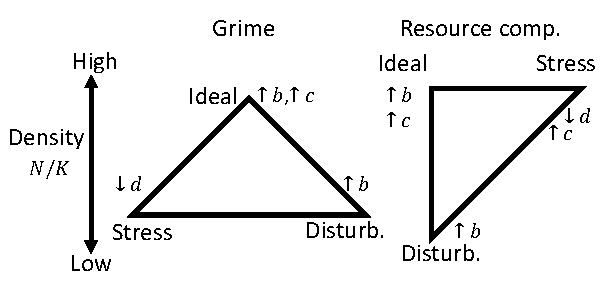
\includegraphics[scale=1]{axes.pdf}
\caption{\label{fig:axes} The realization of Grime's triangle in our model. Schematic representation of the triangular space bounded by the low/high extremes of stress/disturbance. The low-$T$ interpretation of stress is also shown. The vertices of the triangles correspond to different environmental extremes. Selection favors different traits at each vertex, leading to different trait clusters.} 
\end{figure}

How does Fig.~4 compare to empirical analyses of Grime's C/S/R strategies? In our comparison we will stick to fishes, corals and plants, for which three-way primary strategy schemes are well developed \citep{grime_1977,winemiller_1992,darling_2012}. The connection of our model to fish strategies is necessarily more tentative, given that fishes are motile and not all territorial. 

In disturbed environments, we predict evolution for higher $b$ and lower $d$, but not higher $c$. Higher $b$ means higher fecundity and/or dispersal ability (see ``Model''). This is consistent with a ruderal strategy. Plant ruderals devote a large proportion of their productivity to seed production \citep{grime_1977}, whereas the analogous ``opportunist'' fishes have large intrinsic growth rates \citep{winemiller_1992}. In corals, ruderals are distinguished by brood spawning (rather than broadcast spawning; \citealt{darling_2012}). This corresponds to higher parental investment and lower overall propagule production --- counter-intuitively, a stereotypical ``$K$-selected'', high-density trait \citep{pianka_1970}. However, since broadcast spawners are vulnerable to an Allee effect at the egg fertilization stage \citep{knowlton_2001}, brood spawning could actually be a way to ensure high $b$ at low densities \citep{darling_2012}. Lower $d$ could be achieved by improved individual resistance to physical destruction, but it is hard to reduce mortality in the face of severe disturbances. Alternatively, shortening the time to reproductive maturity (the iteration time in our model) is an effective way of reducing the chance of death per iteration, $d$, for a given frequency of disturbance. An exceptionally short life cycle is probably the most defining characteristic of ruderals \citep{grime_1977,winemiller_1992,darling_2012}. Note that if evolution manages to appreciably reduce $d$ for a given disturbance intensity, then the population no longer lies at the extreme disturbance vertex of Grime's triangle. Thus, ruderals are characterized by both high $b$ and high $d$, but there is a constant pressure for a shorter life cycle, extending the limits of disturbance that can be tolerated. 

In stressful environments, we predict evolution for lower $d$, and also  for higher $c$ in the high-density interpretation of stressful environments. Low $d$ is essential when $b\ll 1$, and stress tolerant plants and corals have long life spans, allowing for long intervals between successful recruitments (and episodic broadcast spawning in corals). For fishes, the ``equilibrium'' strategy is the analogue of Grime's stress tolerator. This strategy is associated with consumable resource limitation, and is also characterized by long life span, as well as high parental investment in tiny broods. This may reflect a high-$c$ strategy in the face of intense competition for severely limited resources (the high-density interpretation).

In ideal environments, we predict evolution for higher $b$ and $c$, but not lower $d$. In plants and corals, a key mechanism for winning territorial contests (higher $c$) is rapidly outgrowing and ``shading out'' competitors; empirically, rapid individual growth is a defining feature of the competitor trait cluster \citep{grime_1977,darling_2012}. The situation for $b$ is more ambiguous. Competitor strategies in plants and corals span a range of $b$. For fishes, the analogous ``periodic'' strategy is characterized by enormous spawn sizes as well as rapid development \citep{winemiller_1992,winemiller_2015}. The role of $b$ in ideal environments will be discussed further below.

\section*{Cyclical birth and death rates}

So we have only considered the low-frequency invasion behavior of Eq. \eqref{eq:master}. Here we start exploring its full time-dependent behaviour. We consider a situation where birth and death rates vary periodically with amplitude sufficent to cause large changes in population density. This is inspired by natural \textit{Drosophila} populations, which expand rapidly in the warmer months when fruit is abundant, but largely die off in the colder months. Within this seasonal population density cycle, hundreds of polymorphisms also cycle in frequency \citep{bergland_14}. Some of these polymorphisms may be adaptive and potentially millions of years old \citep{bergland_14}. In this situation, selection on allele frequencies occurs on the same time scale as population demography, a considerably more complicated scenario than classical sweeps in demographically stable populations \citep{messer_2016}.

In the classical population genetic treatment of fluctuating selection, environmental fluctuations do not promote coexistence. Allele frequencies are successively multiplied by relative fitness values for each environmental iteration, and so two alleles favored in different enviroments can only stably coexist if the product of fitnesses for one type exactly equals the product for the other \citep{dempster_1955}. Thus, stable coexistence still requires frequency dependent selection or heterozygote advantage (as is required in a constant environment). 

One general mechanism which by which fluctuating selection promotes coexistence is the ``storage effect'', which occurs when some individuals are protected from selection, and is would appear as a form of frequency dependent selection in the classical analysis of \cite{dempster_1955}.

. In the lottery model, a certain fraction of the adult population ($(1-d_i)n_i$ of each type) does not experience selection in a given iteration. This favors rare types more than abundant ones, because abundant types 

 
 


Figure \ref{fig:fluctuatingselection} shows the behavior of Eq. \eqref{eq:master} for an example where $b$ and $d$ cycle between zero and positive values (``summers'' with rapid growth and no mortality, and ``winters'' with mortality and no growth). Two types are present, a $b$ specialist, which is better at rapidly growing in the summer (higher $b$), and a $d$ specialist which is better at surviving the winter (lower $d$).  Neither type has an advantage over a full environmental cycle, and they stably coexist. Stable coexistence was not possible in a constant environment (section ``''), and occurs in Fig. \ref{fig:fluctuatingselection} due to the storage effect. 





 
Current approaches to population genetic inference treat demography and selection separately, typically fitting a demographic model to data on ostensibly neutral sites, and then inferring selection against this demographic background, despite the recurrent problem that the two are confounded \citep{schrider_2016}. in expanding (e.g. humans) or seasonally-cycling (e.g. . 








 
\begin{figure}
\centering
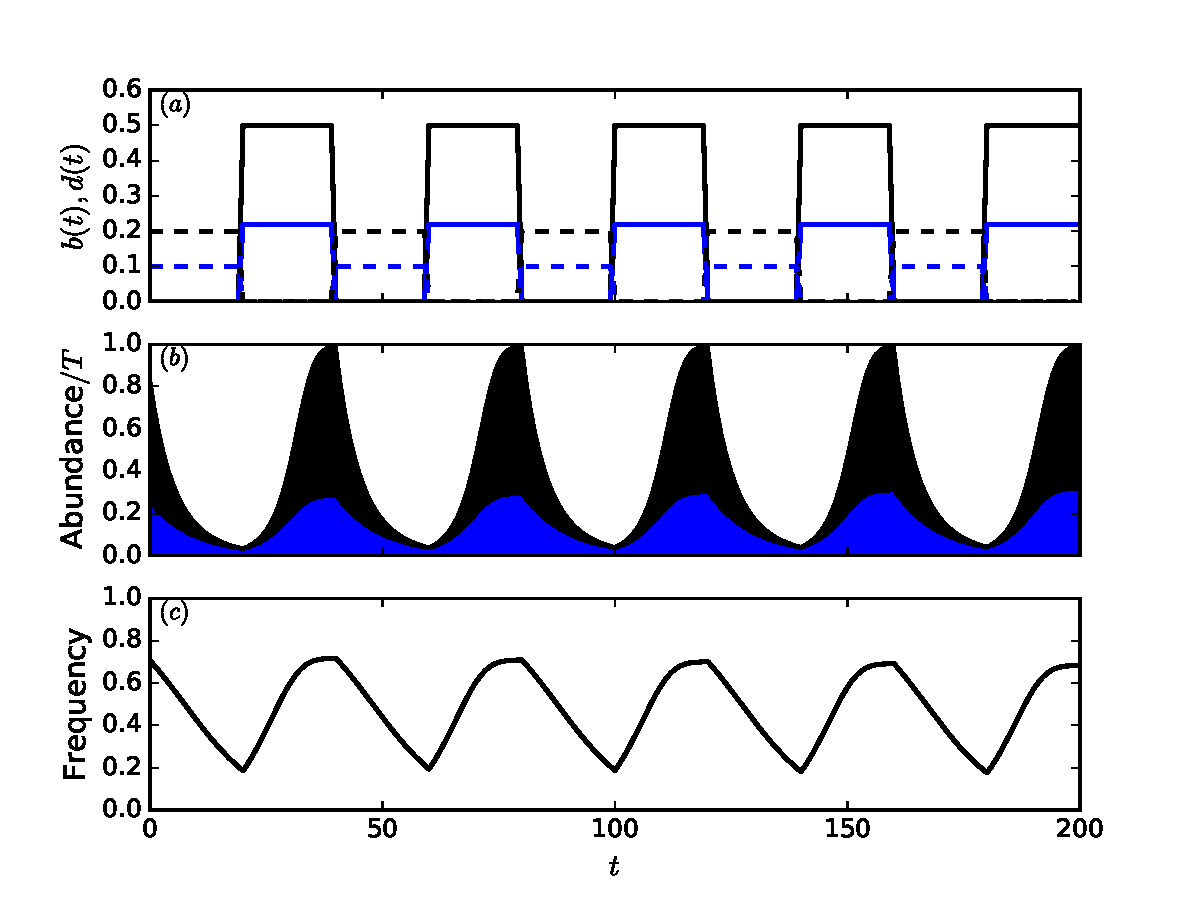
\includegraphics[scale=0.7]{fluctuatingselection.pdf}
\caption{\label{fig:fluctuatingselection} Stable coexistence between $b$ and $d$ specialists when $b$ and $d$ fluctuate. (a) $b$ (solid lines) and $d$ (dashed lines) alternate being nonzero. The $b$ specialist (black) has higher $b$ and $d$ than the $d$ specialist (blue). (b) Both types grow during the positive $b$ phase, and decline during the positive $d$ phase, but the $d$ specialist (blue) does so at a slower rate than the $b$ specialist (black). Total height (blue+black) is population size $N$. (c) The positive $b$ and $d$ phases favor the $b$ and $d$ specialists, respectively, and they stably coexist due to the storage effect.} 
\end{figure}

\section*{Discussion}

As discussed in ``Primary strategies and Grime's triangle'', adaptive evolution in the direction predicted by our generalized lottery model produces traits consistent with Grime's scheme, with the possible exception of selection for $b$ at high density, because the corresponding trait data  is ambiguous. Selection for $b$ at high density is also is counter to the expectations of MacArthur's $r$/$K$ dichotomy \citep{macarthur_1967}, since $b$ is closely related to the maximal, low-density growth rate $r=b-d$ \citep{pianka_1972}, yet in the $r$/$K$ scheme, high density populations should be subject to $K$, not $r$, selection. 

It is not surprising that $b$ can matter at high densities. In our model (or any lottery model of competition), $b$ matters at high densities because territorial contests among juveniles are intrinsically unpredictable. This is a realistic feature of the model. Even if one genotype is guaranteed to win a territory in a ``fair'' contest (e.g. it is the most efficient exploiter of a limiting consumable resource; \citealt{tilman_1982}), inferior competitors can win by chance. For example, an inferior competitor's propagules may happen to arrive first, gaining a decisive developmental advantage. First arrivals are more likely to occur for genotypes with a fecundity and/or dispersal advantage, as represented by higher $b$ in lottery models. The analogous intuition in the Wright-Fisher model is that fecundity confers a relative fitness advantage, even though population size is not changing. The logistic model for which $r$ and $K$ are named, does not capture this intuition. 

Confusingly, the term ``$K$-selection'' sometimes refers generally to selection at high density \citep{pianka_1972}, encompassing both selection for higher saturation density \citep{macarthur_1967} and competitive ability \citep{gill_1974}. Contrary to an $r$/$K$ dichotomy, empirical studies have shown that maximal growth rate and saturation density (measured by abundance) are positively correlated, both between species/strains \citep{luckinbill_1979,kuno_1991,hendriks_2005,fitzsimmons_2010}, and as a result of experimental evolution \citep{luckinbill_1978,luckinbill_1979}. From the perspective of our model, this correlation is not surprising since the saturation density, which is determined by a balance between births and deaths, increases with $b$.

There is support for a negative relationship between competitive success at high density and maximal growth rate \citep{luckinbill_1979}, consistent with an $r$/$K$ dichotomy. This could be driven by a tradeoff between individual size and reproductive rate. To avoid confusion with other forms of ''$K$-selection'', selection for competitive ability has been called ``$\alpha$-selection'' after the competition coefficients in the Lotka-Volterra equation \citep{gill_1974,case_1974,joshi_2001}. However, competitive success as measured by $\alpha$ (i.e. the per-capita effect of one genotype on another genotype's growth rate) is only partly determined by individual competitive ability --- in the presence of age-structured competition and territoriality, it also includes the ability of each genotype to produce contestants i.e. $b$ in our model. Our $c$ is strictly competitive ability only --- as such, changes in $c$ do not directly affect population density (section ``Model''). The clean separation of a strictly-relative $c$ parameter is particularly useful from an evolutionary genetics perspective, essentially embedding a zero-sum relative fitness trait within a non-zero-sum fitness model. This could have interesting applications for modeling the impacts of intra-specific competition on species extinction, for example due to clonal interference \citep{gerrish_1998,desai_2007} between $c$-strategists on the one hand, and $b$- and $d$- strategists on the other.

$K$-selection in the narrow logistic sense of selection for a greater environmental carrying capacity for given birth and death rates, sometimes referred to as ``efficiency'' \citep{macarthur_1967}, could be represented in our model by smaller individual territorial requirements. To a first approximation, two co-occurring genotypes which differ by a small amount in their territorial requirements only should have the same fitness since the costs or benefits of a change in the amount of unocupied territory is shared equally among genotypes via the propagule density per territory $L$. The situation is more complicated when the differences in territorial requirements become large enough that territorial contests can occur on different scales for different genotypes. We leave these complications for future work.

In the classic lottery model, $b_i$ and $c_i$ are essentially equivalent in the sense that the number of territorial victories only depends on the product $b_i c_i$ (see ``Model''). This is no longer the case in our density- and frequency-dependent generalization, where $b$ and $c$ specialists can co-exist. This ``colonization-competition trade-off'' is well known in the co-existence literature \citep{tilman_94}. It and similar forms of ``spatial co-existence'' in stable environments have previously been modeled either with Levin's  qualitative representation of competition \citep{levins_71,tilman_94}, as opposed to the quantitative $c$ of lottery competition, or with a more sophisticated treatment of space (non-uniform dispersal; \citealt{shmida_84,bolker_99}). In fluctuating environments our model would likely give similar co-existence predictions as \cite{chesson_1981}, which revolve around the ``storage effect'', since we retain overlapping generations and competition at the juvenile phase only. 

Our realization of Grime's triangle (Fig.~4) differs from approaches which identify primary strategies as trait combinations which can co-exist \citep{bolker_99}, referring instead to the direction of adaptive trait evolution under different regimes of stress and disturbance, which is closer in spirit to Grime's arguments \citep{grime_1974,grime_1977}. In addition, we have not assumed any kind of trade-offs or pleitropy between $b$, $c$ and $d$, only constraints imposed by the environment on the order of magnitude of $b$ and $d$. As an example of a trade-off, corals which rapidly out-shade neighbors have a tall, branched morphology which is vulnerable to disturbances, and so, all else being equal, ideal environment $c$-strategists will suffer higher mortality from disturbances \citep{darling_2012}. Fig.~\ref{fig:axes} gives the same conclusion without invoking trade-offs; mutations which reduce disturbance vulnerability are essentially neutral under ideal conditions, leading to no improvements in mortality from disturbances, whereas $c$ will tend to increase over time. Thus, while trade-offs may amplify specialization, and are sometimes invoked to explain primary strategy schemes \citep{macarthur_1967,winemiller_1992,aerts_1999}, they are not necessary for it.

%In Fig. \ref{fig:table2} we compare our model with some of the other models and schemes touched upon here. In a sense this is an ``apples and oranges'' comparison: for instance, Grime's scheme was developed for an entirely different purpose (species classification by traits). As such, Fig. \ref{fig:table2} is not exhaustive and should be read more as a summary of our model's purpose. Like MacArthur's $r$/$K$ scheme, our model is motivated by the need to expand the treatment of selection in population genetics \citep{macarthur_1962}, i.e. to incorporate crucial ecological factors in our most genetically realistic models of evolution. Thus, viewing evolutionary ecology \citep{kokko_2007,pelletier_2009,schoener_2011} as a spectrum ranging from evolution-only to ecology-only, our model lies close to the understudied evolution-only end of the spectrum. By comparison, more familiar approaches to evolutionary ecology such as adaptive dynamics --- essentially ecology coupled with mutant invasion \citep{diekmann_2004} ---  lie close to the ecology-only end of the spectrum. 

%\begin{figure}
%\centering
%\begin{tabularx}{\linewidth}{lXXXXX}
%&Formal model?  & Ecologically meaningful? & Empirically-grounded trait scheme? & Generality beyond specific scenarios? & Genetically flexible? \\ \hline
%Density-dependent lottery & \ding{51} & \ding{51} & \ding{51} & \ding{51} & \ding{51} \\  
%  MacArthur's $r$/$K$ + $\alpha$ & \ding{51} & \ding{51} & \ding{55}* & \ding{51} & \ding{51} \\
%  Grime's C/S/R & \ding{55} & \ding{51} & \ding{51} & \ding{51} & NA \\
%  Traditional pop. gen. & \ding{51} & \ding{55} & \ding{55} & \ding{51} & \ding{51} \\
%  Eco-evo:  \\
%  \quad Adaptive dynamics & \ding{51} & \ding{51} & \ding{51} & \ding{51}** & \ding{55} \\
%  \quad Brute force simulation & \ding{51} & \ding{51} & NA & \ding{55} & \ding{51}
%\end{tabularx}
%\caption{\label{fig:table2} Comparison of our density-dependent lottery model with related models and schemes in ecology and evolutionary biology. *MacArthur's $r$- and $K$-, as well as $\alpha$ selection, were all derived theoretically. Applications to traits came later, and with mixed success (see ``Introduction'' and ``Discussion''). **In practice, most of the adaptive dynamics literature focuses on specific eco-evolutionary outcomes such as evolutionary ``branching'' \citep{geritz_1997} or mutualisms \citep{ferriere_2002}, but in principle it can be applied with any fitness model including our density-dependent lottery.}
%\end{figure}

One limitation of our model as a general-purpose model of density-dependent selection is the restriction of competition to interference competition between juveniles for durable resources (lottery recruitment to adulthood), analogous to the ubiquitous assumption of viability selection in population genetics \citep[p. 45]{ewens_2004}. In some respects this is the complement of resource competition models, which restrict their attention to exploitation competition, typically without age structure \citep{tilman_1982}. In the particular case that resources are spatially localized (e.g. due to restricted movement through soils), resource competition and territorial acquisition effectively coincide, and in principle resource competition could be represented by a competitive ability $c$ (or conversely, $c$ should be derivable from resource competition). The situation is more complicated if the resources are well-mixed, since, in general, resource levels then need to be explicitly tracked. It seems plausible that explicit resource tracking may not be necessary when the focus is on the evolution of similar genotypes rather than the stable co-existence of widely differing species \citep{ram_2016}. We are not aware of any attempts to delineate conditions under which explicit resource tracking is unnecessary even if it is assumed that community structure is ultimately determined by competition for consumable resources. More work is needed connecting resource competition models to the density-dependent selection literature, since most of the former has to date been focused on narrower issues of the role of competition at low resource availability \citep{aerts_1999,davis_1998,tilman_2007}.  

While our model can be applied to species rather than genotypes (e.g. ecological invasions), our focus is genotype evolution. Our assumption that there are no large $c$ discrepancies (section ``Mean field approximation'') amounts to a restriction on the amount of genetic variation in $c$ in the population. Since beneficial mutation effect sizes will typically not be much larger than a few percent, large $c$ discrepancies can only arise if the mutation rate is extremely large, and so the assumption will not be violated in most cases. However, this restriction could become important when looking at species interactions rather than genotype evolution.

%\section*{Acknowledgments}

%We thank Peter Chesson and Joachim Hermisson for many constructive comments on this manuscript. This work was financially supported by the National Science Foundation (DEB-1348262).

\bibliographystyle{amnatnat}
\bibliography{reference} 

\section*{Appendix A: Poisson approximation}

For each genotype's dispersal, the counts of propagules across unnocupied territories follows a multinomial distribution with equal probabilities of landing in each territory. Thus, the $x_i$ in different territories are not independent random variables. However, for sufficiently large $T$, holding $n_i/T$ fixed, the Poisson limit theorem implies that this multinomial distribution for the $x_i$ accross territories is closely approximated by a product of independent Poisson distributions for each territory, each with rate parameter $l_i$ (large $T$ implies large $U$ except in the biologically uninteresting case that there is vanishing population turnover $d_i \sim 1/T$). 

Alternatively, we could have assumed a Poisson distribution for the $x_i$ as our model of dispersal from the outset. The total number of genotype $i$ propagules $\sum x_i$ (summed over unoccupied territories) would then no longer be a constant $m_i$, but would fluctuate between generations for a given mean $m_i$, which is more biologically realistic. Nevertheless, for simplicity and ease of comparison with the classic lottery model, we ignore the possibility of fluctuations in $m_i$ and focus instead on Poisson fluctuations propagule composition in each territory. 

\section*{Appendix B: Derivation of growth equation}

We separate the right hand side of Eq.~\eqref{eq:growthsumuncoupled} into three components $\Delta_+ n_i = \Delta_u n_i+\Delta_r n_i+\Delta_a n_i$ which vary in relative magnitude depending on the propagule densities $l_i$. Following the notation in the main text, the Poisson distributions for the $x_i$ (or some subset of the $x_i$) will be denoted $p$, and we use $P$ as a general shorthand for the probability of particular outcomes.

\subsection*{Growth without competition}

The first component, $\Delta_u n_i$, accounts for territories where only one focal propagule is present $x_i=1$ and $x_j=0$ for $j\neq i$ ($u$ stands for ``uncontested''). The proportion of territories where this occurs is $l_i e^{-L}$, and so 
\begin{equation}
\Delta_u n_i=Ul_i e^{-L}=m_i e^{-L}.
\end{equation}

\subsection*{Competition when rare}

The second component, $\Delta_r n_i$, accounts for territories where a single focal propagule is present along with at least one non-focal propagule ($r$ stands for ``rare'') i.e. $x_i=1$ and $X_i\geq 1$ where $X_i=\sum_{j\neq i} x_j$ is the number of nonfocal propagules. The number of territories where this occurs is $Up_i(1)P(X_i\geq 1)=b_i n_i e^{-l_i}(1-e^{-(L-l_i)})$. Thus 
\begin{equation}
\Delta_r n_i = m_i e^{-l_i}(1-e^{-(L-l_i)})\left\langle  \frac{c_i}{c_i +\sum_{j\neq i} c_j x_j } \right\rangle_{\tilde{p}},  \label{eq:deltr}
\end{equation}
where $\langle \rangle_{\tilde{p}}$ denotes the expectation with respect to $\tilde{p}$, and $\tilde{p}$ is the probability distribution of nonfocal propagule abundances $x_j$ \textit{after} dispersal, in those territories where exactly one focal propagule, and at least one non-focal propagule, landed. 

Our ``mean field'' approximation is to replace $x_j$ with its mean in the last term in Eq.~\eqref{eq:deltr},
\begin{equation}
\left\langle\frac{c_i}{c_i +\sum_{j\neq i} c_j x_j}\right\rangle_{\tilde{p}}\approx \frac{c_i}{c_i +\sum_{j\neq i} c_j \langle x_j\rangle_{\tilde{p}}}.\label{eq:meanfieldr}
\end{equation}
Below we justify this replacement by arguing that the standard deviation $\sigma_{\tilde{p}}(\sum_{j\neq i} c_j x_j)$ (with respect to $\tilde{p}$), is much smaller than $\langle\sum_{j\neq i} c_j x_j\rangle_{\tilde{p}}$.

We first calculate $\langle x_j \rangle_{\tilde{p}}$. Let $X=\sum_j x_j$ denote the total number of propagules in a territory and ${\mathbf x_i}=(x_1,\ldots,x_{i-1},x_{i+1}\ldots,x_G)$ denote the vector of non-focal abundances, so that $p({\mathbf x_i})=p_1(x_1)\ldots p_{i-1}(x_{i-1})p_{i+1}(x_{i+1})\ldots p_G(x_G)$. Then, $\tilde{p}$ can be written as
\begin{align}
\tilde{p}({\mathbf x_i})&=p({\mathbf x_i}|X\geq 2,x_i=1)\nonumber\\
&=\frac{P({\mathbf x_i},X\geq 2|x_i=1)}{P(X\geq 2)}\nonumber\\
&=\frac{1}{1-(1+L)e^{-L}}\sum_{X=2}^{\infty} P(X) p({\mathbf x_i}|X_i=X-1),
\end{align}
and so
\begin{align}
\langle x_j \rangle_{\tilde{p}}&=\sum_{\mathbf x_i} \tilde{p}({\mathbf x_i})x_j\nonumber\\
&=\frac{1}{1-(1+L)e^{-L}}\sum_{X=2}^{\infty} P(X) \sum_{\mathbf x_i} p({\mathbf x_i}|X_i=X-1)x_j.
\label{eq:raremonster1}
\end{align}
The inner sum over ${\mathbf x_i}$ is the mean number of propagules of a given nonfocal type $j$ that will be found in a territory which received $X-1$ nonfocal propagules in total, which is equal to $\frac{l_j}{L-l_i}(X-1)$. Thus, 
\begin{align}
\langle x_j \rangle_{\tilde{p}}&=\frac{l_j}{1-(1+L)e^{-L}}\frac{1}{L-l_i}\sum_{k=2}^{\infty} P(X) (X-1)\nonumber\\
&=\frac{l_j}{1-(1+L)e^{-L}}\frac{L-1+e^{-L}}{L-l_i},
\label{eq:meanxjrare}
\end{align}
where the last line follows from $\sum_{X=2}^{\infty} P(X)(X-1)=\sum_{X=1}^{\infty} P(X)(X-1)=\sum_{X=1}^{\infty} P(X)X-\sum_{X=1}^{\infty}P(X)$.

The exact analysis of the fluctuations in $\sum_{j\neq i} c_j x_j$ is complicated because the $x_j$ are not independent with respect to $\tilde{p}$. These fluctuations are part of the ``drift'' in type abundances which we leave for future work. Here we use the following approximation to give some insight into the magnitude of these fluctuations and also the nature of the correlations between the $x_j$. We replace $\tilde{p}$ with $\tilde{q}$, defined as the ${\mathbf x_i}$ Poisson dispersal probabilities conditional on $X_i\geq1$ (which are independent). The distinction between $\tilde{p}$ with $\tilde{q}$ will be discussed further below. The $\tilde{q}$ approximation gives $\langle x_j \rangle_{\tilde{q}}=\langle x_j \rangle_p/C=l_j/C$, 
\begin{align}
\sigma_{\tilde{q}}^2(x_j)&=\langle x_j^2 \rangle_{\tilde{q}}-\langle x_j \rangle_{\tilde{q}}^2\nonumber\\
&=\frac{1}{C}\langle x_j^2 \rangle_p-\frac{l_j^2}{C^2}\nonumber \\
&=\frac{1}{C}(l_j^2 + l_j)-\frac{l_j^2}{C^2}\nonumber \\
&=\frac{l_j^2}{C}\left(1-\frac{1}{C}\right)+\frac{l_j}{C},\label{eq:varr}
\end{align}
and 
\begin{align}
\sigma_{\tilde{q}}(x_j,x_k)&=\langle x_j x_k \rangle_{\tilde{q}}-\langle x_j \rangle_{\tilde{q}}\langle x_k \rangle_{\tilde{q}}\nonumber\\
&=\frac{1}{C}\langle x_j x_k \rangle_p-\frac{l_jl_k}{C^2}\nonumber\\
&=\frac{l_j l_k}{C}\left(1-\frac{1}{C}\right),\label{eq:covr}
\end{align}
where $C=1-e^{-(L-l_i)}$ and $j\neq k$. 

The exact distribution $\tilde{p}$ assumes that exactly one of the  propagules present in a given site after dispersal belongs to the focal type, whereas $\tilde{q}$ assumes that there is a focal propagule present before non-focal dispersal commences. As a result, $\tilde{q}$ predicts that the mean propagule density is greater than $L$ (in sites with only one focal propagule is present) when the focal type is rare and the propagule density is high. This is erroneous, because the mean number of propagules in every site is $L$ by definition. Specifically, if $L-l_i \approx L\gg 1$, then the mean propagule density predicted by $\tilde{q}$ is approximately $L+1$. The discrepancy causes rare invaders to have an intrinsic rarity disadvantage (territorial contests under $\tilde{q}$ are more intense than they should be). In contrast, Eq. \eqref{eq:meanxjrare} correctly predicts that there are on average $\sum_{j\neq i}\langle x_j \rangle_{\tilde{p}}\approx L-1$ nonfocal propagules because $\tilde{p}$ accounts for potentially large negative covariances between the $x_j$ ``after dispersal''. By neglecting the latter covariences, $\tilde{q}$ overestimates the fluctuations in $\sum_{j\neq i} c_j x_j$; thus $\tilde{q}$ gives an upper bound on the fluctuations. The discrepancy between $\tilde{q}$ and $\tilde{p}$ will be largest when $L$ is of order $1$ or smaller, because then the propagule assumed to already be present under $\tilde{q}$ is comparable to, or greater than, the entire propgaule density. 

Decomposing the variance in $\sum_{j\neq i} c_j x_j$,
\begin{equation}
\sigma_{\tilde{q}}^2(\sum_{j\neq i} c_j x_j)=\sum_{j\neq i}\left[c_j^2\sigma_{\tilde{q}}^2(x_j)+2\sum_{k>j, k\neq i}c_j c_k\sigma_{\tilde{q}}(x_j,x_k)\right],\label{eq:vartotr}
\end{equation}
and using the fact that $\sigma_{\tilde{q}}(x_j,x_k)$ and the first term in Eq. \eqref{eq:varr} are negative because $C<1$, we obtain an upper bound on the relative fluctuations in $\sum_{j\neq i} c_j x_j$, 
\begin{equation}
\frac{\sigma(\sum_{j\neq i} c_j x_j)}{\langle\sum_{j\neq i} c_j x_j\rangle}=C^{1/2}\frac{\left(\sum_{j\neq i}c_j^2 l_j+(1-1/C)\left(\sum_{j\neq i}c_j l_j\right)^2 \right)^{1/2}}{\sum_{j\neq i}c_j l_j}<C^{1/2}\frac{\left(\sum_{j\neq i}c_j^2 l_j\right)^{1/2}}{\sum_{j\neq i}c_j l_j}. \label{eq:cvr}
\end{equation}

Suppose that the $c_j$ are all of similar magnitude (their ratios are of order one). Then Eq.~\eqref{eq:cvr} is $\ll 1$ for the case when $L-l_i \ll 1$ (due to the factor of $C^{1/2}$), and also for the case when at least some of the nonfocal propagule densities are large $l_j\gg 1$ (since it is then of order $1/\sqrt{L-l_i}$). The worst case scenario occurs when $L-l_i$ is of order one. Then Eq.~\eqref{eq:cvr} gives a relative error of approximately $50\%$, which from our earlier discussion we know to be a substantial overestimate when $L$ is of order $1$. Our numerical results (Fig. \ref{fig:simcomp}) confirm that the relative errors are indeed small.

However, the relative fluctuations in $\sum_{j\neq i} c_j x_j$ can be large if some of the $c_j$ are much larger than the others. Specifically, in the presence of a rare, extremely strong competitor ($c_j l_j\gg c_{j'} l_{j'}$ for all other nonfocal genotypes $j'$, and $l_j\ll 1$), then the RHS of Eq. \eqref{eq:cvr} can be large and we cannot make the replacement Eq.~\eqref{eq:meanfieldr}. 

Substituting Eqs. \eqref{eq:meanfieldr} and \eqref{eq:meanxjrare} into Eq.~\eqref{eq:deltr}, we obtain
\begin{equation}
\Delta_r n_i\approx m_i R_i\frac{c_i}{\overline{c}}, \label{eq:deltrfinal}
\end{equation}
where $R_i$ is defined in Eq.~\eqref{eq:Dr}.

\subsection*{Competition when abundant}

The final contribution, $\Delta_a n_i$, accounts for territories where two or more focal propagules are present ($a$ stands for ``abundant"). Similarly to Eq.~\eqref{eq:deltr}, we have 
\begin{equation}
\Delta_a n_i=U(1-(1+l_i)e^{l_i})\left\langle \frac{c_i x_i}{\sum_j c_j x_j} \right\rangle_{\hat{p}}\label{eq:delta}
\end{equation}
where $\hat{p}$ is the probability distribution of both focal and nonfocal propagaule abundances \textit{after} dispersal in those territories where at least two focal propagules landed. 

Again, we argue that the relative fluctuations in $\sum c_j x_j$ are much smaller than $1$ (with respect to $\hat{p}$), so that,
\begin{equation}
\left\langle \frac{c_i x_i}{\sum_j c_j x_j} \right\rangle_{\hat{p}}\approx  \frac{c_i \langle x_i \rangle_{\hat{p}}}{\sum_j c_j \langle x_j\rangle_{\hat{p}}}.\label{eq:meanfielda}
\end{equation}
Following a similar procedure as for $\Delta_r n_i$, where the vector of propagule abundances is denoted ${\mathbf x}$, the mean focal genotype abundance is, 
\begin{align}
\langle x_i \rangle_{\hat{p}}&=\sum_{\mathbf x} x_i p(\mathbf x|x_i\geq 2)\nonumber \\
&=\sum_{x_i} x_i p(x_i|x_i\geq 2) \nonumber\\
&=\frac{1}{1-(1+l_i)e^{-l_i}}\sum_{x_i\geq 2} p(x_i)x_i\nonumber\\
&=l_i\frac{1-e^{-l_i}}{1-(1+l_i)e^{-l_i}}.
\end{align}
For nonfocal genotypes $j\neq i$, we have
\begin{align}
\langle x_j \rangle_{\hat{p}}&=\sum_{\mathbf x} x_j p(\mathbf x|x_i\geq 2)\nonumber \\
&=\sum_{X}P(X|x_i\geq 2)\sum_{\mathbf x} x_j p({\mathbf x}|x_i\geq 2,X)\nonumber\\
&=\sum_{X}P(X|x_i\geq 2)\sum_{x_i} p(x_i|x_i\geq 2,X) \sum_{\mathbf x_i} x_j p(\mathbf x_i|X_i=X-x_i)\nonumber\\
&=\sum_{X}P(X|x_i\geq 2)\sum_{x_i}p(x_i|x_i\geq 2,X) \frac{l_j(X-x_i)}{L-l_i} \nonumber\\
&=\frac{l_j}{L-l_i}\left[\sum_{X}P(X|x_i\geq 2)X - \sum_{x_i}p(x_i|x_i\geq 2) x_i \right]\nonumber\\
&=\frac{l_j}{L-l_i}\left( L\frac{1-e^{-L}}{1-(1+L)e^{-L}}- l_i\frac{1-e^{-l_i}}{1-(1+l_i)e^{-l_i}}\right). 
\end{align}

To calculate the relative fluctuations in $\sum_{j\neq i} c_j x_j$, we use a similar approximation as for $\Delta_r n_i$: $\hat{p}$ is approximated by $\hat{q}$, defined as the ${\mathbf x}$ dispersal probabilities in a territory conditional on $x_i>2$ (that is, treating the $x_j$ as indepenent). All covariances between nonfocal genotypes are now zero, so that $\sigma_{\hat{q}}^2(\sum c_j x_j)=\sum c_j^2 \sigma_{\hat{q}}^2(x_j)$, where $\sigma_{\hat{q}}^2(x_j)=l_j$ for $j\neq i$, and  
\begin{equation}
\sigma_{\hat{q}}^2(x_i)=\frac{l_i}{D}\left(l_i+1-e^{-l_i}-\frac{l_i}{D}\left(1-e^{-l_i}\right)^2\right),
\end{equation}
where $D= 1-(1+l_i)e^{-l_i}$, and 
\begin{equation}
\frac{\sigma_{\hat{q}}(\sum c_j x_j)}{\langle\sum c_j x_j\rangle} = \frac{\left(\sum_{j\neq i} c_j^2 l_j + c_i^2 \sigma_{\hat{q}}^2(x_i)\right)^{1/2}}{\sum_{j\neq i} c_j l_j + c_i l_i (1-e^{-l_i})/D} \label{eq:cva}.
\end{equation}

Similarly to Eq.~\eqref{eq:cvr}, the RHS of Eq. \eqref{eq:cva} is $\ll 1$ for the case that $L \ll 1$ (due to a factor of $D^{1/2}$), and also for the case when at least some of the propagule densities (focal or nonfocal) are large --- provided that $c_i$ and the $c_j$ are all of similar magnitude. Again, the worst case scenario occurs when $l_i$ and $L-l_i$ are of order $1$, in which case Eq. \eqref{eq:cva} is around $35\%$, which is again where the $\hat{q}$ approximation produces the biggest overestimate of the fluctuations in ${\mathbf x}$. Similarly to Eq.~\eqref{eq:cvr}, the RHS of \eqref{eq:cva} will not be $\ll 1$ in the presence of a rare, extremely strong competitor.  

Combining Eqs. \eqref{eq:delta} and \eqref{eq:meanfielda}, we obtain
\begin{equation}
\Delta_a n_i=m_i A_i \frac{c_i}{\overline{c}},
\end{equation}
where $A_i$ is defined in Eq.~\eqref{eq:Da}.

%\subsection{Logistic growth and classic nesting sites model}

%In the nesting sites model, it is assumed that propagules landing on occupied territory do not survive, while those landing on unoccupied territory immediately occupy the territory. Thus, the probability that a propagule survives is simply $(1-N/K)$, where $N=\sum_i n_i$ is the total population size. Consequently, $n_i$ increases by $1$ over the interval $[t,t+\Delta t]$ with probability $b_i n_i (1-N/K)\Delta t$. Provided that the abundances $n_i$ are large enough that demographic stochasticity is negligible (i.e. they have established), we can treat $n_i(t)$ as a continuous variable with growth given by the expectation of $b_i n_i (1-N/K)\Delta t$, and so, taking $\Delta t \rightarrow 0$ we obtain
%\begin{equation}
%\frac{dn_i}{dt}=b_i\left(1-\frac{N}{K}\right)n_i. \label{eq:logistic}
%\end{equation}

%\section{Territorial availability}
%
%In Sec. \ref{sec:c} we assumed that adults have the same territorial requirement, regardless of genotype. This can be generalized to allow genotypes to differ in their territorial requirements. Each adult from genotype $i$ now requires $t_i$ units of territory, $T$ is the total territory available to the population, and $T-\sum_i t_i$ units of territory are unoccupied. 
%
%Competition between propagules with different territorial requirements is potentially much more complicated than the model in Sec. \ref{sec:c}, because competition is no longer neatly partitioned into a set of identical territories.  The larger a propagule's territorial requirement, the more neighboring propagules it will interact with during its development to adulthood. 
%
%
%A simple way to avoid these complications is to partition the unoccupied territory into uniform units of territory with size given by the largest territorial requirement $t^*={\rm max}_i t_i$. The uniform territory approach used in Sec.  \ref{sec:c}
%
%The biological intuition behind this 
%
%Thus $U=(T-\sum_i t_i n_i)/t^*$.


\end{document}
